%!TEX root = ../main.tex
\section{Evaluation}
\label{sec:evaluation}
% 
In this section, we evaluate the performance of Rime. First, we describe our test environment in Section~\ref{subsec:test_env}. Then, we introduce our emulation setup in Section~\ref{sec:evaluation-line-rate}.
After that, we evaluate different aspects of Rime, i.e., failure recovery in Section~\ref{sec:evaluation-failure-recovery}, efficient query dissemination in Section~\ref{sec:evaluation-query-dissemination}, scalability and maintenance overhead in Section~\ref{sec:evaluation-scalability-and-maintenance}, and the support of geo-spatial movement of nodes in Section~\ref{sec:evaluation-movement}.
For the sake of reproducibility, we release Rime as well as experiment configurations in a public repository.~\footnote{https://github.com/jo-jstrm/rime-data-streaming-iot}

\subsection{Test Environment}
\label{subsec:test_env}
% 
Our test environment consists of emulated nodes deployed on a single server. All benchmarks were performed on a server with Ubuntu 18.04 on an Intel Xeon E5620 (2.4GHz) CPU with 47GiB memory. 
The hardware resources of the server allows for emulating topologies with sizes up to $73$ nodes. Table~\ref{tab:experiment-configuration} lists all the topologies used throughout our experiments. We found that topologies larger than $T_{73}$ degrade performance on the host due to hardware limitations.
%\steffen{maybe say before performance or so degenerate}
We use a tree-like topology with configurable \texttt{height} and \texttt{degree} across all experiments.
For node emulation, we use Containernet~\cite{peuster_medicine_2016}, 
a network emulator that is an extension of Mininet~\cite{lantz_network_2010} which is capable of running 
Docker~\footnote{https://docker.com} containers. This setup allows for flexible deployment 
of nodes or experiments and supports emulating node failures in a reproducible manner. We utilize emulation rather than network simulators since simulators use models to represent the current environment, hence they abstract details for the sake of accuracy. A network emulator on the other hand leads to easier testing on a diverse set of hardware and allows for faster and prototyping~\cite{symeonides2020fogify}.

\textbf{Assumptions} In order to evaluate our approach, we make some simplifications about our running environment. In all our tests we assume that the root node does not fail. 
One possible solution to root node failures would be a consensus mechanism that can be utilized in order to elect a new root between candidates. However, we argue that a root could be hosted within a cloud and thus exclude this aspect from the following considerations.

\textbf{Baseline} To the best of our knowledge, there exists no open-sourced implementation of 
SRTs that is suitable as a baseline for our evaluation. 
The closest is TinyDB~\cite{madden2005tinydb} that was part of TinyOS in a single release that is not available anymore.\footnote{http://telegraph.cs.berkeley.edu/tinydb/software.html} TinyOS and its \texttt{nesc} compiler are not further developed and have transitioned to getting volunteer updates.\footnote{https://github.com/tinyos/tinyos-main}
Therefore, we compare Rime to a baseline-system that connects nodes using an immutable routing tree.
We consider this to be a suitable baseline with low maintenance-overhead at the cost of no failure recovery and update propagation. To implement the baseline, we compile Rime without any SRT-features, i.e., no parent-selection algorithm, backup parent, and state-tracking of remote nodes. This ensures that Rime and the baseline are as similar as possible. We elaborate further on our baseline assumptions and practicalities in Section~\ref{sec:evaluation-line-rate}.

\textbf{Running Example}\label{Running Example.} Figure~\ref{fig:basic-srt} shows the 
running example topology that we use for our experiments. 
The tree resulting from this topology has a $height$ of three, which is the highest number of hops on the path from root to leaf. Furthermore, it has a $degree$ of two, which is the number of children of each node, including the root. The node IDs are allocated using breadth-first search. 
For our experiments in Section~\ref{sec:evaluation-scalability-and-maintenance}, we extend this basic topology by increasing height and degree, as well as the number of nodes. We show the resulting
deployment configurations in Table~\ref{tab:experiment-configuration}.
The geo-spatial location for all nodes is randomly assigned within the interval $\{latitude, longitude\}\in(0.0,100.0)\textrm{ meters}$ of a uniform distribution created with an MT19937 random number generator.\footnote{https://www.cplusplus.com/reference/random/mt19937/} In Section~\ref{sec:evaluation-failure-recovery} and Section~\ref{sec:evaluation-query-dissemination} experiments start after location assignment and parent selection are complete. This is necessary to let Rime propagate updates and create an SRT. 
%\johannes{I do not really get this sentence. Do we want to emphasize that we artificially set location in the BEGINNING? Or do we want to say that we give Rime enough time before experiments 4.3 and 4.4 start?}. 
For all experiments, we set the sampling rate of each sensor at every node to two tuples per second, which is common in WSNs~\cite{madden2005tinydb, akyildiz2002wireless}.
% \steffen{please say why exactly these frequency maybe claim at least it is common or so}

\begin{table}[t]
  \centering
  \caption{Experiment configurations used for evaluation.}
  \vspace{-3mm}
  \begin{tabular}{| c | c | c | c |}
    \hline
    \textbf{ID} & \textbf{$\#$ of Nodes} & \textbf{Degree} & \textbf{Height} \\
    \hline
    $T_{7}$ & 7 & 2 & 2 \\
    \hline
    $T_{13}$ & 13 & 3 & 2 \\
    \hline
    $T_{15}$ & 15 & 2 & 3 \\
    \hline
    $T_{21}$ & 21 & 4 & 2 \\
    \hline
    $T_{40}$ & 40 & 3 & 3 \\
    \hline    
    $T_{73}$ & 73 & 8 & 2 \\
    \hline    
  \end{tabular}
\label{tab:experiment-configuration}
\end{table}

\subsection{Exploration of Emulation Boundaries}
\label{sec:evaluation-line-rate}
As a first step for our evaluation, we test the maximum throughput and average latency of our setup with the baseline system over a static topology. This provides a practical line rate when the system only performs routing of tuples from the edge to the cloud nodes, without applying processing. Edge nodes do not move or change location and the keep producing two tuples per second (t/s) uninterrupted.  
We observe the average combined incoming 
throughput at the sink of the query is 146 t/s. 
% Throughput is directly proportional to the number of 
% generated tuples in each node, since there are no failures.\steffen{what do you want to say here is this a statement?} 
The average latency of a single packet traveling from an edge node
to the base station is 96.5 milliseconds (ms). This is in line with the randomized latency that
we insert in the topology through the emulator, where we use a random latency range of [60-150]ms for the edge nodes and [10-30]ms for parents to base-station.

In a second experiment, we evaluate the cost of node failure due to movement with the baseline. Recall that the baseline has Rime features turned off, thus there is no way for a disconnected node to recover. 
%\steffen{In general could you not call the baseline Tinydb-like or so to really make clear that this is used there?}
%\dimi{We couldn't really call it Tinydb-like, since it would require only multi-hop comm and message stealing. This is much work to implement and the reason we're going with this approach (we explain that we never found its implementation).}
The impact of node movement is directly proportional to the size of the sub-tree of the failing nodes. %\steffen{this is really hard to follow}
As an example, on a tree with $degree=8$ and $height=2$, if a node at $height=1$ 
fails, then the whole sub-tree is disconnected from the network; thus the network loses ~$\approx\frac{1}{8}$ of the nodes. We provide details about the cost of recovering from failure using Rime in Section~\ref{sec:evaluation-failure-recovery}.

\subsection{Failure Recovery}\label{sec:evaluation-failure-recovery}
% \steffen{be nice to the reader, provide a smooth transition into the section}
In this experiment, we explore how Rime performs recovery from failure, even if the node is a parent.
Failure of a parent node disconnects all its children from the rest of the tree.
Therefore, no sensor readings from the affected subtree can reach the sink. Rime offers a coping mechanism for parent-failure through backup parents. The backup parent is the second best candidate from the parent selection process.

To quantify the ability of Rime to recover from failures, we measure the \textit{recovery latency}.
We define the recovery latency as the time between the failure of one or several nodes and the point in time when regular operation resumes, i.e., the successful registration of all children of the failed node to their backup parents.
We use the same base topology $T_7$ as the running example in Section~\ref{subsec:test_env} and
we measure the recovery latencies of 10 runs when either node $1$ or node $2$ fails.
%\steffen{somehow you are talking about an experiment is there no figure? can we describe the setup better somehow?}
In each run, we let the parent with most children fail, such that a failure has the highest possible impact on Rime. Throughout the experiment, the recovery latency varies between $46ms$ and $366ms$, with a median of $201.5ms$. We account the variations of the recovery latency to \textit{1)} the varying number of queued messages at the receiver and \textit{2)} scheduling on the emulating host. 
% 
% We observe that with the median recovery latency\steffen{what does that mean? when it occurs? I am confused}, all children of the disconnected node lose at most one sensor reading per failure, assuming constant throughput per second per node. 
Recovery from node failure is not possible in the baseline-system, whereas Rime timely reconnects the nodes. Thereby, Rime resumes routing with insignificant tuple loss after a failure.

% \johannes{old content, keep it for the numbers} Throughout the experiment, the recovery latency $l$ varies between $l_{min}=46ms$ and $l_{max}=366ms$, with mean $\bar l=178.5ms$ and median $\bar l_{med}=201.5ms$. The interquartile range is $127.25ms$ and reaches from $96.5ms$ to $223.75ms$. We account the variations of the recovery latency to \textit{i)} the varying number of queued messages at the receiver and \textit{ii)} scheduling on the emulating host. Assuming a recovery latency of $\bar l_{med}=201.5ms$, the children of the disconnected node lose at most one tuple per failure with a constant throughput of two tuples per second per node. This is not possible in the baseline, where there is no coping mechanism for failures. Rime timely reconnects the nodes and routing resumes with minimal tuple loss.
% \steffen{I am lost, what do you want to tell me here, please say it explicitly and also summarize what this means for the rest of the paper, the reader, and everything else}

\begin{table}[t]
  \centering
  \caption{Baseline messaging-overhead compared Rime for different selectivities. Rime significantly reduces the number of messages needed to get a query to all applying nodes.}
  \vspace{-3mm}
  \begin{tabular}{| c | c | c | c|}
    \hline
    \textbf{Selectivity} &  \begin{tabular}[c]{@{}c@{}}\textbf{Baseline}\\ \textbf{Overhead} \end{tabular} &  \begin{tabular}[c]{@{}c@{}}\textbf{Rime}\\ \textbf{Overhead} \end{tabular} & \begin{tabular}[c]{@{}c@{}}\textbf{Rime} \\ \textbf{Savings}\end{tabular}\\
    \hline
    $10\%$ & $87.67\%$ & $5.02\%$ & $82.65\%$ \\
    \hline
    $25\%$ & $70.32\%$ & $1.83\%$ & $68.49\%$ \\
    \hline
    $80\%$ & $24.20\%$ & $2.74\%$ & $21.46\%$ \\
    \hline
  \end{tabular}
\label{tab:query-results}
\end{table}

\subsection{Efficient Query Dissemination}
\label{sec:evaluation-query-dissemination}
% 
% \steffen{need a good transition here}
In this experiment, we quantify how efficiently Rime filters out unnecessary nodes for a query. A key benefit of using SRTs in Rime is its ability to discard whole subtrees of a query if the nodes in a subtree do not contain relevant values. 
To evaluate the benefit of this characteristic, we measure the overhead of Rime as well as the baseline in Table~\ref{tab:query-results}. The overhead is defined as the ratio of the number of nodes that received the query and the number of nodes that have relevant data for the query.
% 
Our query selects values from all location sensors installed at the nodes, inside a 2D area. 
We use topology $T_{40}$ and vary query-selectivitiy, i.e., number of nodes participating in the query, between $10\%$, $25\%$, and $80\%$. 
Table~\ref{tab:query-results} presents the average overhead for each selectivity.
As shown, Rime reduces the average overhead by up to $82.65\%$. This means that Rime performs better for queries with a lower selectivity. The main reason is that Rime is able to choose only relevant nodes for a query, which is emphasized in queries with low selectivities. The results indicate that the overhead of Rime is minimal compared to the baseline.
% In particular, Rime needs parent nodes to forward the query to the sources and the parents are not necessarily equipped with sensors or they do not report relevant data for the query.\steffen{I am confused now I don't know what you want to say here}

\begin{figure}[t]
  \centering
  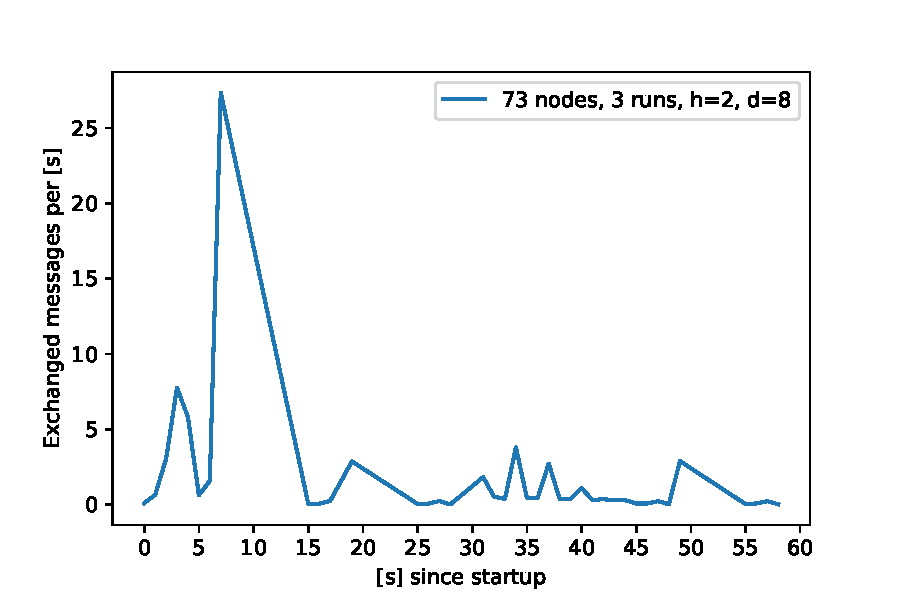
\includegraphics[width=0.5\textwidth]{img/evaluation/vliot/movement-avg-msgs-per-node-73.pdf}
  \caption{Message transmissions per node of $T_{73}$. The spikes starting after 31s shows the number of transmissions during a stepwise tree-attribute change.}
  \label{fig:movement-avg-per-node}
\end{figure} 

\subsection{Scalability and Maintenance Overhead}
\label{sec:evaluation-scalability-and-maintenance}
%
Building and maintenance of SRTs require message exchange between nodes, which is the main cost of building an SRT. To determine the required message transmissions, we measure the number of exchanged messages per second in Rime during the first minute after start-up. To determine the scalability of Rime, we use data from all topologies detailed in Table~\ref{tab:experiment-configuration}. We choose $T_{73}$ as an example for showing the behavior of Rime \textit{during} and \textit{after} startup. We use the largest topology to fully show the effects of scalability in Rime. Figure~\ref{fig:movement-avg-per-node} shows the average number of exchanged messages per second over three runs using $T_{73}$.
The communication peak during the first $10s$ stems from the initial data exchange and the requests from children for parent selection. The reoccurring local maximum of message transmissions at $20s$, $35s$, and $50s$ originate from the regular collection of the current tree topology. 
%Through this information collection, we observe how the network evolves over time with Rime.\steffen{where? and why are you saying this here?}
Furthermore, we discuss the peaks at $31s$, $34s$, and $37s$ in Section~\ref{sec:evaluation-movement}, as they are related to node movement.

%\johannes{TODO: Make a decision on whether to keep Figure 6 or not, because it is redundant with Table 3.} 
Across all topologies, we identify spikes of message transmissions until $15s$ after startup. Figure~\ref{fig:avg-overhead-per-node} shows the sum of exchanged messages \textit{per node} for all topologies during the first $20s$, such that we account for all startup spikes. This way we account for the overhead of extra messages needed to build and update the SRT in the same time-frame.
%\steffen{? what does this mean}. 
We observe that the messaging overhead increases with topology size. 
As shown in Table~\ref{tab:total-messages}, topology $T_{73}$ induces the overall maximum number of messages.
However, topology $T_{73}$ induces less messages per node than $T_{40}$, even though $T_{73}$ contains more nodes.  This is due to the larger height of $T_{40}$, which leads to a larger pool of candidate parents. Thus, $T_{40}$ induces more parent selection messages. We observe that the height of the tree is another important factor to message overhead, which can dominate in topologies with complex structure. 
% \steffen{I think what you need to say here is that the common belevie is that with increasing number of nodes the number of messages increase but you show that this is not alon true and thus also the height or topology or strucutre play a role}
%\steffen{I am still ask myself what is the diff between t7 and t55 I think the number of nodes but I am not sure}
Table~\ref{tab:total-messages} shows that the average increase in transmissions per node is near to linear, under the same height.
Furthermore, the number of transmissions stays low, with periodical spikes during topology collection. Comparing the messaging overhead of $2.86$ messages per node per second with $T_{40}$ with the throughput of modern SPEs, which is magnitudes higher~\cite{zeuch2019analyzing}, we find the overhead negligible.
% to the we find the messaging overhead of $2.86$ messages per node per second with $T_{40}$ to be negligible.\steffen{I don't know what you want to say here and it sounds rather negative to me} %\dimi{change this to per second per node, so it looks smaller}
%\steffen{mh this sentence sounds weird and I cannot agree by just reading what you wrote}

\begin{table}[t]
  \centering
  \caption{Message statistics for all topologies, taken from the first 20s after startup.}
  \vspace{-3mm}
  \begin{tabular}{| c | c | c | c |}
    \hline
    \textbf{ID} & \textbf{Total} & \textbf{Messages} & \textbf{Messages} \\
     & \textbf{Messages} &  \textbf{per node} &  \textbf{per second per node} \\
    \hline
    $T_{7}$ & 175 & 25.12 & 1.26 \\
    \hline
    $T_{13}$ & 454 & 34.90 & 1.74 \\
    \hline
    $T_{15}$ & 563 & 37.54 & 1.88 \\
    \hline
    $T_{21}$ & 841 & 40.04 & 2.00 \\
    \hline
    $T_{40}$ & 2292 & 57.29 & 2.86 \\
    \hline    
    $T_{73}$ & 3721 & 50.97 & 2.55 \\
    \hline    
  \end{tabular}
\label{tab:total-messages}
\end{table}

\subsection{Geo-spatial Movement of Nodes}\label{sec:evaluation-movement}
In this experiment, we measure the number of exchanged messages in a dynamic environment, where nodes change their positions. In this experiment we move a node step-wise, where each step is an increase of latitude and longitude by three meters within the space defined in the running example in Section~\ref{subsec:test_env}. Rime needs to account for movement in order to maintain efficient query dissemination. Movement might change which parent is the closest one for a node. Therefore, each node initializes parent selection after its movement has ended.
%\steffen{what does it mean for rime that a node moves? does it get a close next parent? from where to where does it move etc.}
The overhead induced by parent selection and metadata exchange for topology updates immediately affects the scalability of Rime. 
Figure~\ref{fig:movement-avg-per-node} shows the number of message transmissions per node per second, during runtime. 
%\steffen{in general you have to provide justification for you chosen parameter, they seem to be hand-picked and it is hard to generalize what would happen for other parameters}
The spike at $31s$ marks the beginning of a continuous movement, where five random children nodes move three times during nine seconds, ending at $38s$. The last spike at $40s$ is the parent selection after movement stops. We start movement after $30s$ in order to give Rime enough time to create and populate the tree. The creation process induces a lot of concurrent updates and does not reflect the state of the network during regular runtime.
%\steffen{ok what would happen if not?}
If no movement occurs, Rime exchanges $233.3$ messages ($3.64$ per node) on average with the same topology during the same period. During the interval $(31s,41s)$, where nodes are moving, $1582.3$ messages ($24.7$ per node) are transmitted on average.

In order to further quantify the impact of movement within Rime, we run the same experiment with two different configurations over the topology $T_{73}$. The configurations differ in the number of moving nodes. In the first configuration, we let one node move, where in the second one we increase this number to $10\%$, i.e., seven nodes. During the movement period, the nodes in the first configuration exchange on average $0.37$ messages per node per second. For the second configuration, this number rises to $2.55$. Our results show that the number of exchanged messages per node per second scales linearly with the number of moving nodes.
% \steffen{again what is the baseline and how do you improve, your are just describe your part but do not offer the reader a broader perspective}
% This behavior emphasizes the fact that changes of the tree-attributes are costly and influential on the overall performance of SRTs. We consider this cost negligible compared to the number of tuples a modern node can process per second~\cite{zeuch2019analyzing}.

Overall, Rime drastically increases the efficiency of query dissemination compared to the baseline, as shown in Section~\ref{sec:evaluation-query-dissemination}. Rime can cope with failures in the topology, something that the baseline is not capable of, as well as recover timely. With the addition of the parent selection algorithm, Rime keeps in check the overhead of maintaining an SRT
and allows it to scale up to the number of updates.
Finally, Rime exploits edge resources and multi-scheme communication between physically distant nodes in order to overcome the original limitations in the radio-based transmission design of SRTs.

\begin{figure}[t]
  \label{fig:init-messages}        
  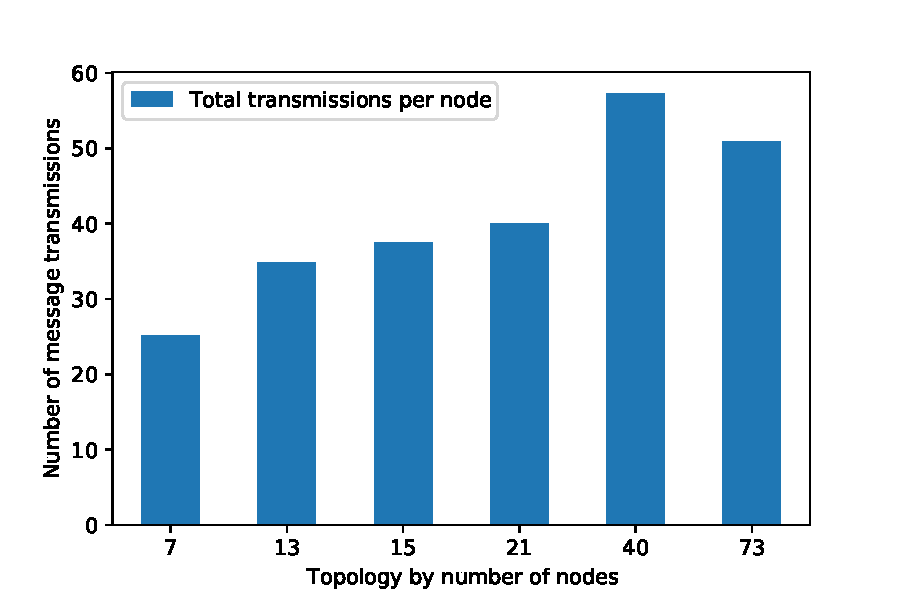
\includegraphics[width=.5\textwidth]{img/evaluation/vliot/maintenance-init-msgs-per-node.pdf}
  \caption{Average number of message transmissions per node during the first 20s of deployment.}
  \label{fig:avg-overhead-per-node}   
\end{figure} 
